\documentclass{article}

\usepackage{amsmath, amssymb, amsfonts}
\usepackage{amsthm}
\usepackage{hyperref}
\usepackage[table]{xcolor}
\usepackage{longtable}
\usepackage{tikz-cd}
\usepackage[paperwidth=6in,paperheight=6in]{geometry}

\newcommand{\N}{\mathbb{N}} 
\newcommand{\Z}{\mathbb{Z}}
\newcommand{\R}{\mathbb{R}} 
\newcommand{\C}{\mathbb{C}}
\newcommand{\D}{\mathcal{D}}
\newcommand{\cO}{\mathcal{O}}
\newcommand{\cP}{\mathcal{P}}
\newcommand{\SO}{\mathrm{SO}}
\newcommand{\Lie}{\mathrm{Lie}}
\newcommand{\g}{\mathfrak{g}}
\newcommand{\q}{\mathfrak{q}}
\newcommand{\h}{\mathfrak{h}}
\newcommand{\fsl}{\mathfrak{sl}}
\newcommand{\fk}{\mathfrak{k}}
\newcommand{\e}{\varepsilon}
\newcommand{\sll}[1]{\mkern-4mu\mathbin{/\mkern-5mu/}_{\mkern-4mu{#1}}}
\newcommand{\slll}[1]{\mkern-4mu\mathbin{/\mkern-5mu/\mkern-5mu/}_{\mkern-4mu{#1}}}
\newcommand{\ft}{\mathfrak{t}}
\newcommand{\s}{\subseteq}
\newcommand{\ip}[1]{\langle #1\rangle}
\newcommand{\too}{\longrightarrow}
\newcommand{\mto}{\mapsto}
\newcommand{\mtoo}{\longmapsto}
\newcommand{\hooklongrightarrow}{\lhook\joinrel\longrightarrow}
\newcommand{\reg}{^{\mathrm{reg}}}
\newcommand{\st}{^{\mathrm{s}}}
\newcommand{\ps}{^{\mathrm{ps}}}
\newcommand{\ass}{^{\textrm{a-ss}}}
\newcommand{\aps}{^{\textrm{a-ps}}}
\DeclareMathOperator{\Span}{span}
\DeclareMathOperator{\Ad}{Ad}
\DeclareMathOperator{\Int}{Int}
\DeclareMathOperator{\rk}{rk}
\DeclareMathOperator{\Spec}{Spec}
\DeclareMathOperator{\Hom}{Hom}

\theoremstyle{plain}
\newtheorem{theorem}{Theorem}[section]
\newtheorem{lemma}[theorem]{Lemma}
\newtheorem{proposition}[theorem]{Proposition}
\newtheorem{corollary}[theorem]{Corollary}
\theoremstyle{definition}
\newtheorem{definition}[theorem]{Definition}
\newtheorem{remark}[theorem]{Remark}
\numberwithin{figure}{section}
\numberwithin{equation}{section}

\newcommand\blfootnote[1]{
  \begingroup
  \renewcommand\thefootnote{}\footnote{#1}
  \addtocounter{footnote}{-1}
  \endgroup
}
\pagenumbering{gobble}

\begin{document}

\topskip0pt

\begin{center}
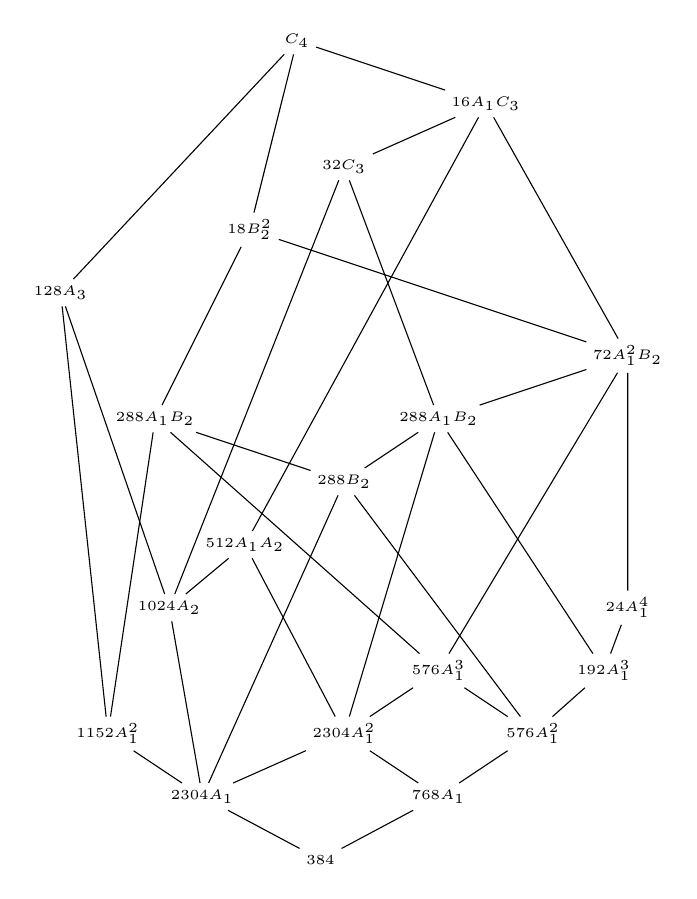
\begin{tikzpicture}[xscale=1.2, yscale=0.8, baseline=(current bounding box.center)]\tiny
\node (9) at (4.5, 13) {$C_4$};
\node (7) at (6.5, 12) {$16A_1C_3$};
\node (12) at (5, 11) {$32C_3$};
\node (10) at (4, 10) {$18B_2^2$};
\node (6) at (2, 9) {$128A_3$};
\node (0) at (8, 8) {$72A_1^2B_2$};
\node (19) at (6, 7) {$288A_1B_2$};
\node (16) at (3, 7) {$288A_1B_2$};
\node (14) at (5, 6) {$288B_2$};
\node (1) at (3.95, 5) {$512A_1A_2$};
\node (15) at (3.15, 4) {$1024A_2$};
\node (8) at (8, 4) {$24A_1^4$};
\node (3) at (7.75, 3) {$192A_1^3$};
\node (2) at (6, 3) {$576A_1^3$};
\node (18) at (2.5, 2) {$1152A_1^2$};
\node (17) at (5, 2) {$2304A_1^2$};
\node (13) at (7, 2) {$576A_1^2$};
\node (5) at (3.5, 1) {$2304A_1$};
\node (4) at (6, 1) {$768A_1$};
\node (11) at (4.75, 0) {$384$};
\draw (6) -- (9);
\draw (3) -- (8);
\draw (8) -- (0);
\draw (0) -- (7);
\draw (15) -- (1);
\draw (0) -- (10);
\draw (19) -- (0);
\draw (13) -- (2);
\draw (15) -- (12);
\draw (4) -- (13);
\draw (16) -- (10);
\draw (11) -- (5);
\draw (5) -- (18);
\draw (17) -- (2);
\draw (18) -- (16);
\draw (10) -- (9);
\draw (2) -- (16);
\draw (17) -- (19);
\draw (11) -- (4);
\draw (14) -- (19);
\draw (5) -- (17);
\draw (12) -- (7);
\draw (17) -- (1);
\draw (18) -- (6);
\draw (3) -- (19);
\draw (7) -- (9);
\draw (14) -- (16);
\draw (13) -- (14);
\draw (13) -- (3);
\draw (4) -- (17);
\draw (5) -- (14);
\draw (2) -- (0);
\draw (15) -- (6);
\draw (5) -- (15);
\draw (19) -- (12);
\draw (1) -- (7);
\end{tikzpicture}
\end{center}



\end{document}

